\documentclass[border=12pt]{standalone}
\usepackage{tikz}
\usetikzlibrary{arrows.meta, shadows, shapes.geometric, positioning}
\usepackage[T1]{fontenc}
\renewcommand{\familydefault}{\sfdefault}

\definecolor{cAI}{HTML}{EA580C}
\definecolor{cAIFill}{HTML}{FFEDD5}
\definecolor{cBackend}{HTML}{7C3AED}
\definecolor{cBackendFill}{HTML}{EDE9FE}
\definecolor{cUser}{HTML}{C026D3}
\definecolor{cUserFill}{HTML}{FAE8FF}
\definecolor{cGreen}{HTML}{16A34A}
\definecolor{cGreenFill}{HTML}{DCFCE7}
\definecolor{cRed}{HTML}{DC2626}
\definecolor{cRedFill}{HTML}{FEE2E2}
\definecolor{cGray}{HTML}{4B5563}
\definecolor{cGrayFill}{HTML}{F3F4F6}

\begin{document}
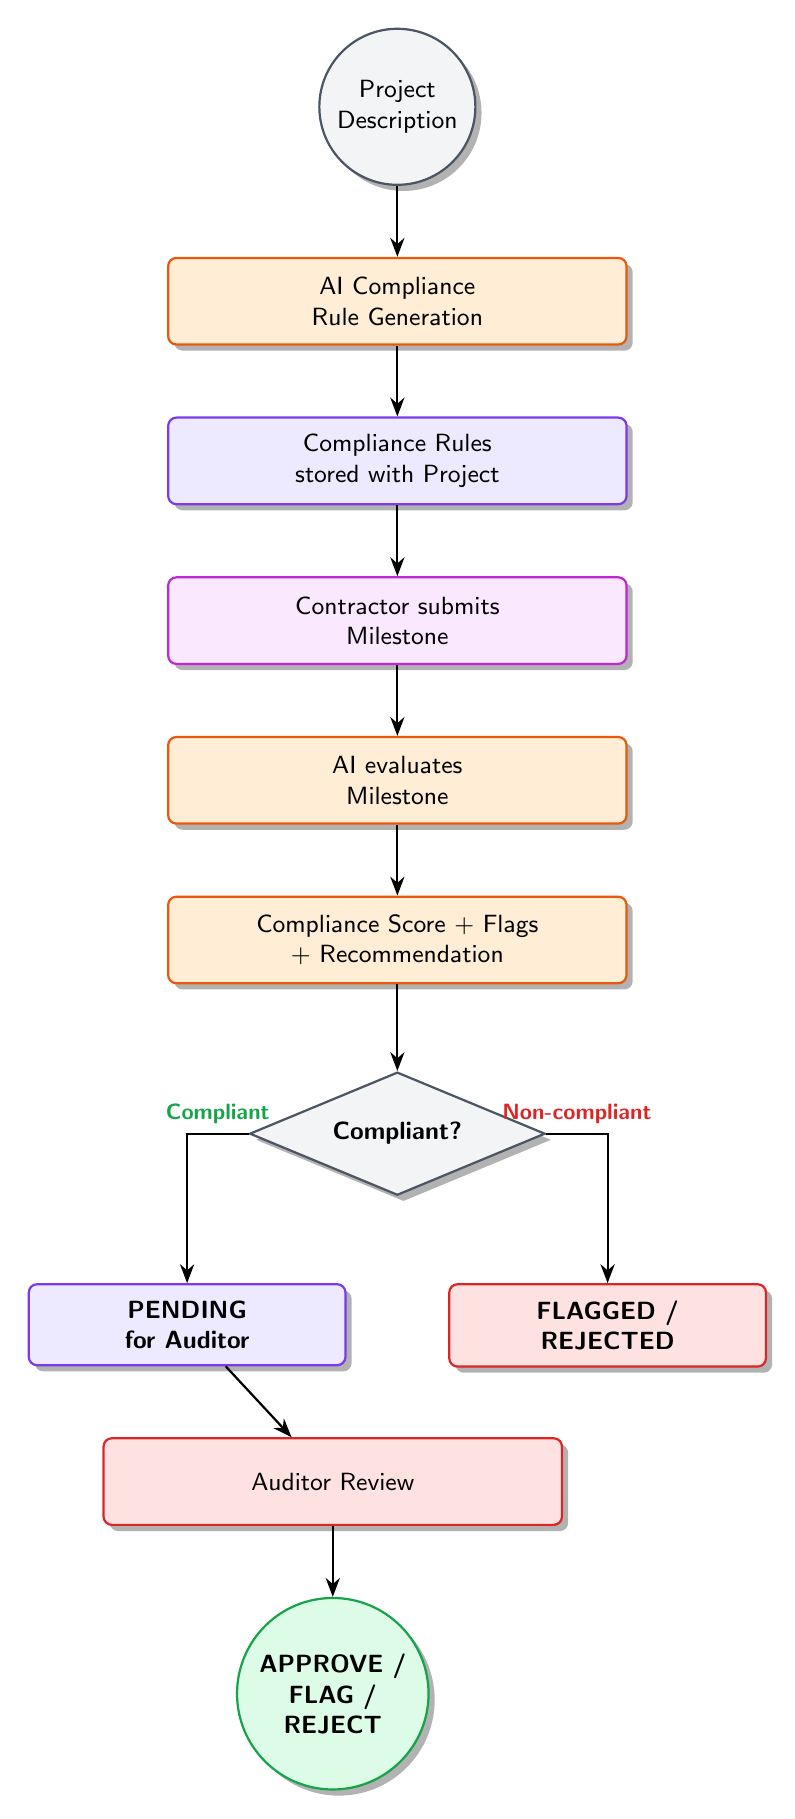
\begin{tikzpicture}[
  node distance=0.9cm and 1.6cm,
  start/.style={circle, draw=cGray, fill=cGrayFill, thick, minimum size=1.9cm,
    font=\small, align=center, drop shadow={opacity=0.3,fill=black}},
  ai/.style={rectangle, rounded corners=3pt, draw=cAI, fill=cAIFill, thick,
    minimum height=1.1cm, text width=5.4cm, align=center, font=\small,
    inner sep=6pt, drop shadow={opacity=0.3,fill=black}},
  backend/.style={rectangle, rounded corners=3pt, draw=cBackend, fill=cBackendFill, thick,
    minimum height=1.1cm, text width=5.4cm, align=center, font=\small,
    inner sep=6pt, drop shadow={opacity=0.3,fill=black}},
  user/.style={rectangle, rounded corners=3pt, draw=cUser, fill=cUserFill, thick,
    minimum height=1.1cm, text width=5.4cm, align=center, font=\small,
    inner sep=6pt, drop shadow={opacity=0.3,fill=black}},
  decision/.style={diamond, draw=cGray, fill=cGrayFill, thick, aspect=2.4,
    text width=2.6cm, align=center, font=\small\bfseries, inner sep=2pt,
    drop shadow={opacity=0.3,fill=black}},
  pending/.style={rectangle, rounded corners=3pt, draw=cBackend, fill=cBackendFill, thick,
    minimum height=1.0cm, text width=3.6cm, align=center, font=\small\bfseries,
    inner sep=6pt, drop shadow={opacity=0.3,fill=black}},
  flagged/.style={rectangle, rounded corners=3pt, draw=cRed, fill=cRedFill, thick,
    minimum height=1.0cm, text width=3.6cm, align=center, font=\small\bfseries,
    inner sep=6pt, drop shadow={opacity=0.3,fill=black}},
  auditor/.style={rectangle, rounded corners=3pt, draw=cRed, fill=cRedFill, thick,
    minimum height=1.1cm, text width=5.4cm, align=center, font=\small,
    inner sep=6pt, drop shadow={opacity=0.3,fill=black}},
  endnode/.style={circle, draw=cGreen, fill=cGreenFill, thick, minimum size=2.1cm,
    font=\small\bfseries, align=center, drop shadow={opacity=0.3,fill=black}},
  arr/.style={-{Stealth[length=2.4mm]}, thick, black},
  glabel/.style={font=\footnotesize\bfseries, text=cGreen},
  rlabel/.style={font=\footnotesize\bfseries, text=cRed}
]

  \node[start] (desc) {Project\\Description};
  \node[ai, below=of desc] (rulegen) {AI Compliance\\Rule Generation};
  \node[backend, below=of rulegen] (store) {Compliance Rules\\stored with Project};
  \node[user, below=of store] (submit) {Contractor submits\\Milestone};
  \node[ai, below=of submit] (evaluate) {AI evaluates\\Milestone};
  \node[ai, below=of evaluate] (score) {Compliance Score + Flags\\+ Recommendation};

  \node[decision, below=1.1cm of score] (decide) {Compliant?};

  \node[pending, below left=1.5cm and -0.3cm of decide] (pending) {PENDING\\for Auditor};
  \node[flagged, below right=1.5cm and -0.3cm of decide] (flagged) {FLAGGED /\\REJECTED};

  \node[auditor, below=of pending, xshift=1.85cm] (review) {Auditor Review};
  \node[endnode, below=of review] (final) {APPROVE /\\FLAG /\\REJECT};

  \draw[arr] (desc)   -- (rulegen);
  \draw[arr] (rulegen)-- (store);
  \draw[arr] (store)  -- (submit);
  \draw[arr] (submit) -- (evaluate);
  \draw[arr] (evaluate)-- (score);
  \draw[arr] (score)  -- (decide);

  \draw[arr] (decide) -| node[glabel, pos=0.25, above] {Compliant} (pending);
  \draw[arr] (decide) -| node[rlabel, pos=0.25, above] {Non-compliant} (flagged);

  \draw[arr] (pending) -- (review);
  \draw[arr] (review)  -- (final);

\end{tikzpicture}
\end{document}
